\documentclass[11pt]{article}

\usepackage[a4paper,top=3cm,bottom=3cm,left=3cm,right=3cm]{geometry}
\usepackage{parskip}		%% blank lines between paragraphs, no indent
\usepackage{amsmath}
\usepackage[utf8]{inputenc}
\usepackage{textcomp}
\usepackage{gensymb}
\usepackage{amssymb}
\usepackage{graphicx}
\newcommand\tab[1][1cm]{\hspace*{#1}}

\begin{document}

\huge \textbf{SaDS HW 3} 
\large \hfill Inti Mendoza \\

\section*{Problem 4.1}

\begin{itemize}
	\item Factorial
	\begin{itemize}
		\item Precondition $P(n)$ is $n \geq 0$ 
		\item Postcondition $Q(n, x)$ is $n \leq x$
		\item Loop invariant $I$ is $product = (factor - 1)!$
		\item Termination orderings is given by $(n-1)!n$	
	\end{itemize}
	\item revertImmutable
	\begin{itemize}
		\item Precondition $P(x)$ is $x \neq \emptyset$
		\item Postcondition $Q(x, rev)$ is $|x| = |rev|$
		\item Loop invariant $I$ is $|rest| = |x| - |rev|$
		\item Termination ordering is given by $rest = \emptyset$
	\end{itemize}
\end{itemize}

\section*{Problem 4.2}

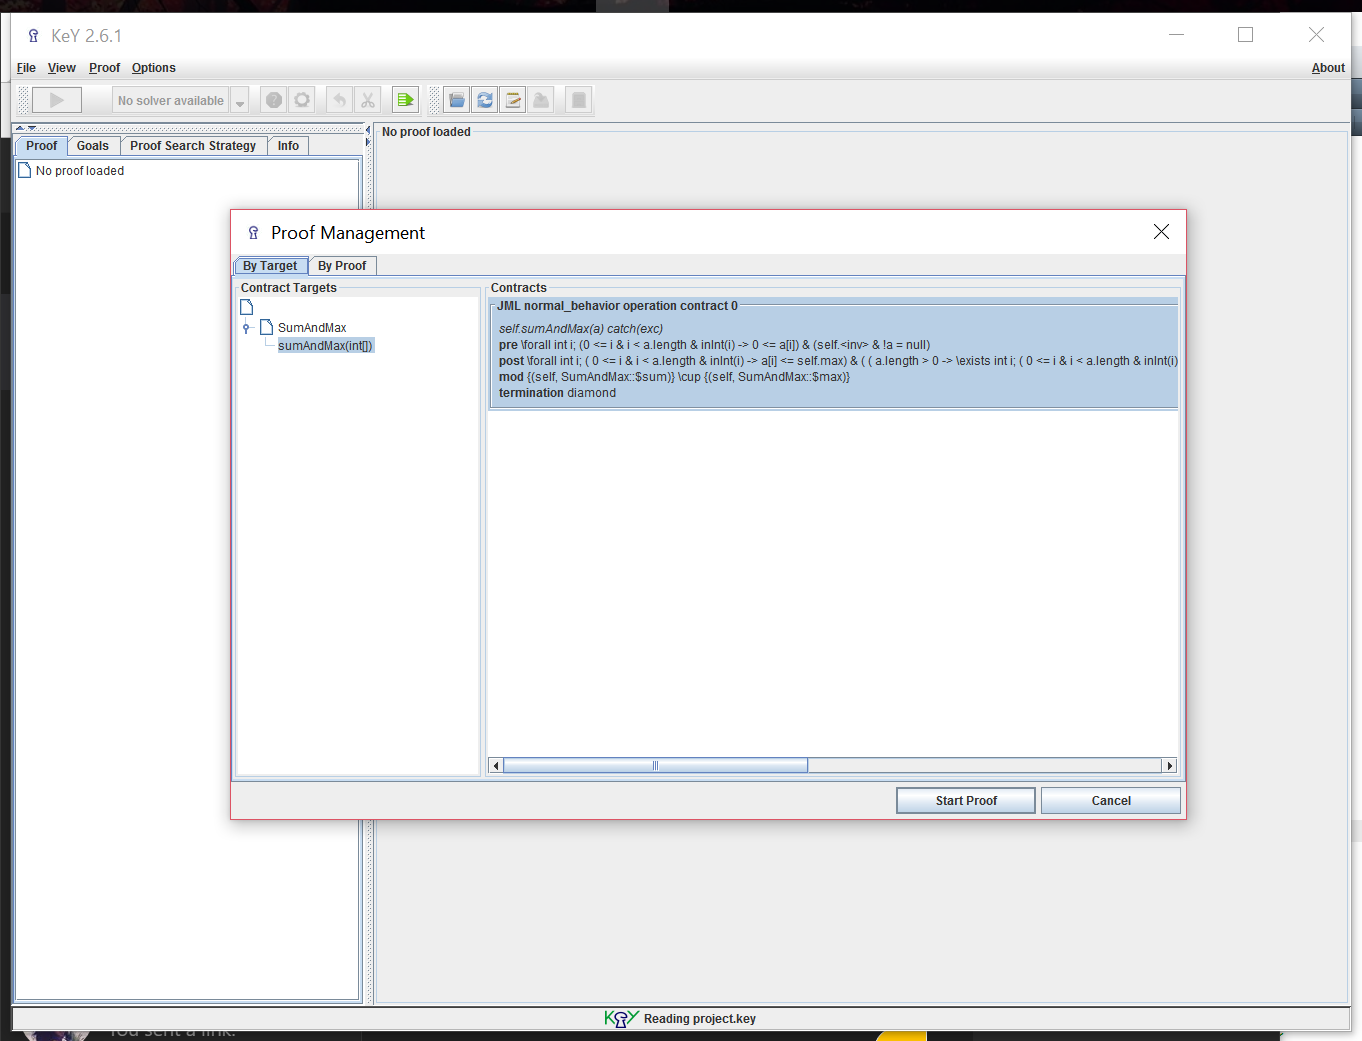
\includegraphics[scale=0.6]{min_max_pre_post.png}\\
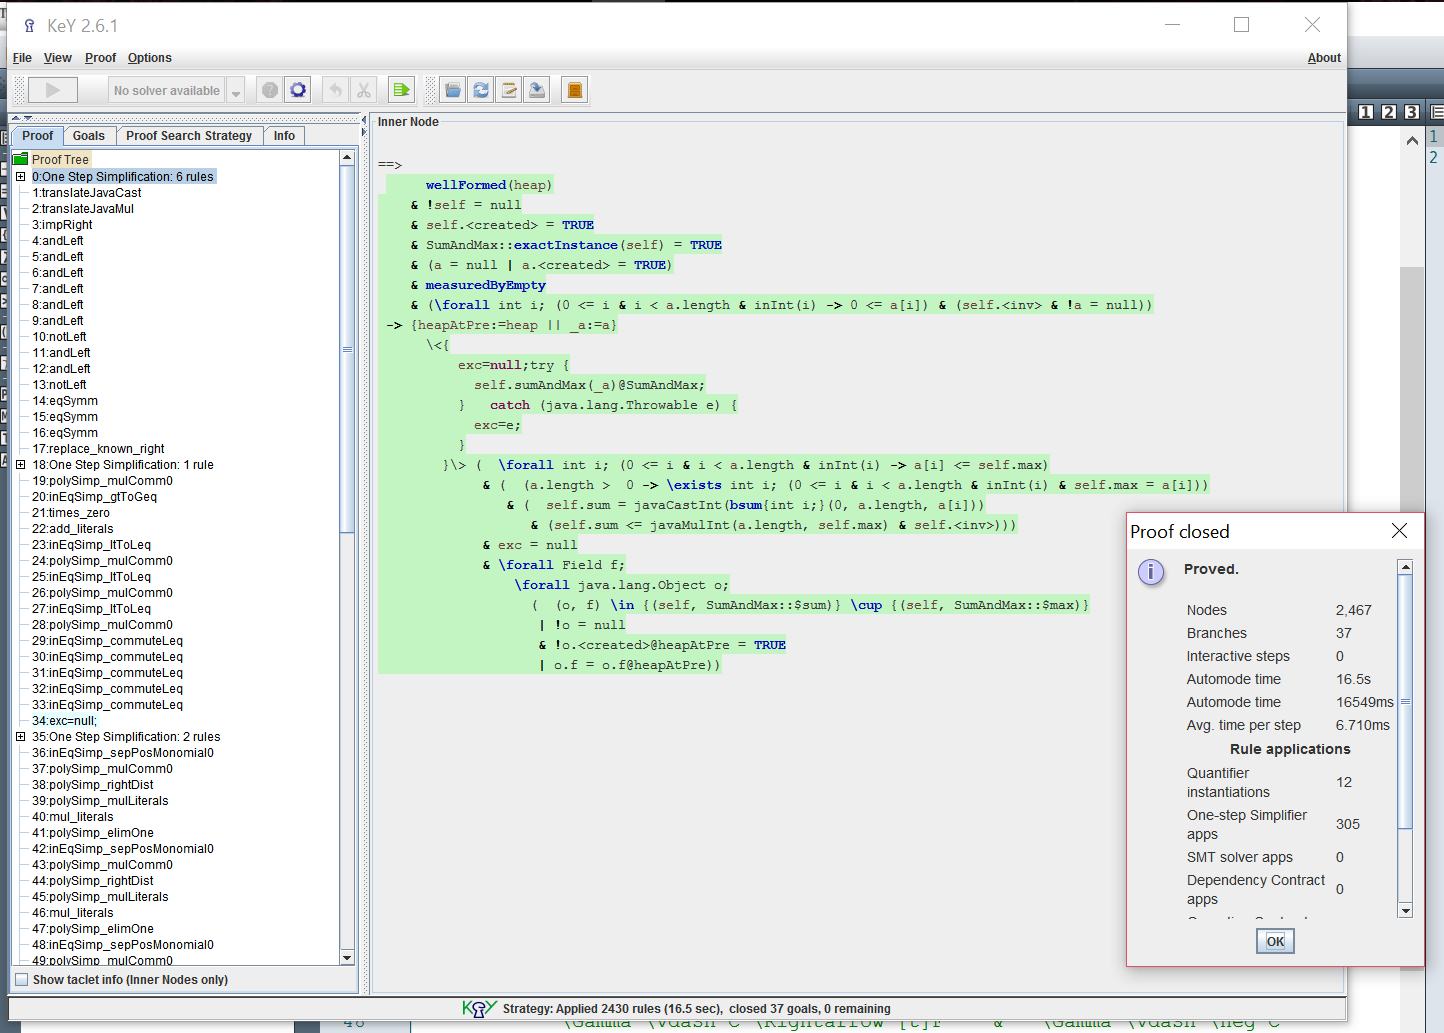
\includegraphics[scale=0.6]{min_max_proof.png} \\ \hline
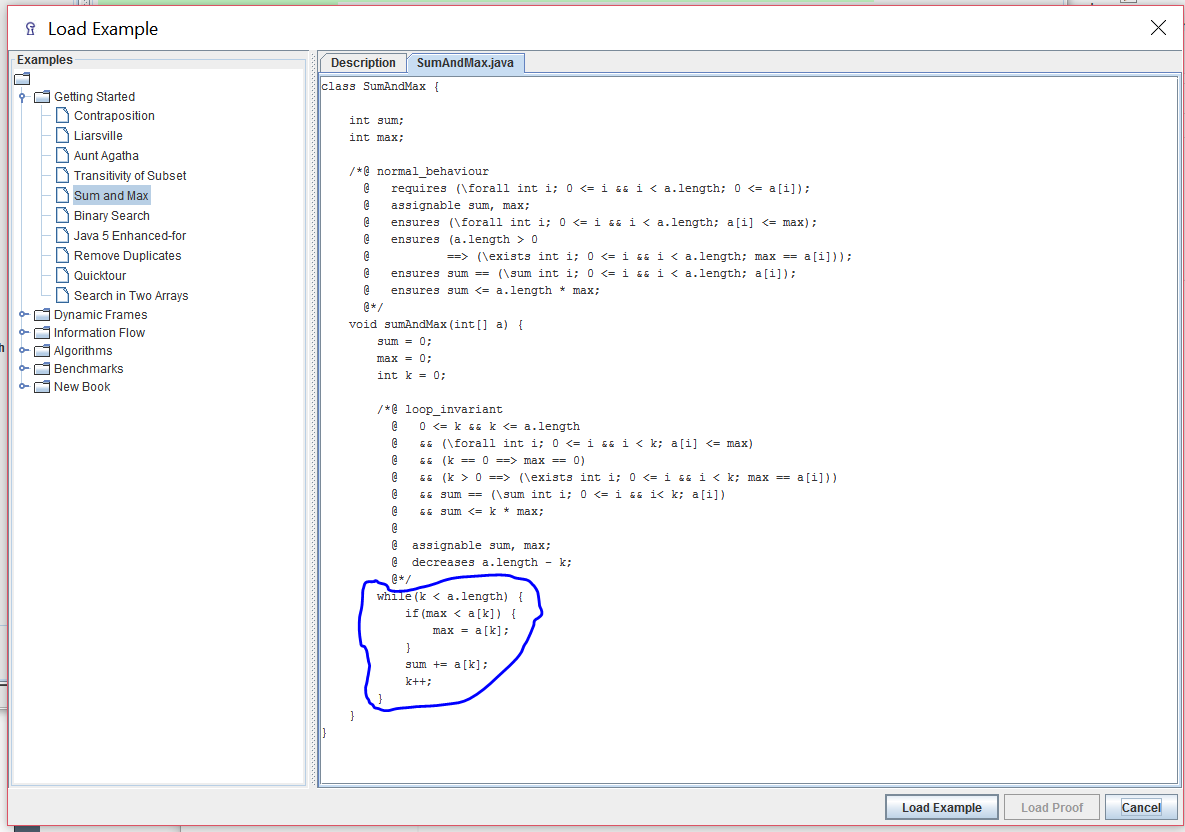
\includegraphics[scale=0.6]{min_max_while.png}

\section*{Problem 4.3}

\begin{itemize}
	\item Proof for soundness of \textbf{if}\\
	\\
	From lecture notes, $C$ is assumed to be pure. Hence, when used in \textbf{if}, every possible outcome has to be true - defined in every state. \textbf{if} produces two cases. When $C == true$ and $C == false$. \\
	In the rule for \textbf{if} : \\
	$
		\begin{matrix}
		\begin{matrix}
			\Gamma \vdash C \Rightarrow [t]F	&	\Gamma \vdash \neg C \Rightarrow [t']F 
		\end{matrix} \\ \hline
		\Gamma \vdash [\textbf{if } (C)\{ t\} \textbf{ else }\{ t'\}]F
		\end{matrix}
	$\\
	C is allowed two states - the states possible by definition of \textbf{if} and is defined in both of them.\\
	$\therefore$ \textbf{if} is sound.
	
	\item Proof for soundness of \textbf{while}\\
	From lecture notes, $C$ is assumed to be pure. Hence, when used in \textbf{while}, every possible outcome has to be true - defined in every state. \textbf{while} has the loop invariant attribute.\\
	In the rule for \textbf{if} : \\
	$
		\begin{matrix}
		\begin{matrix}
		\Gamma \vdash I	&	\Gamma * \vdash (I \land C) \Rightarrow [t]I	&	\Gamma \vdash (I \land \neq C) \Rightarrow F
		\end{matrix} \\ \hline
		\Gamma \vdash [\textbf{while} C \{ t\} ]F
		\end{matrix}
	$\\
	The loop invariant is defined as true before and after \textbf{while} starts for whatever $C$.\\
	$\therefore$ \textbf{while} is sound.
\end{itemize}

\end{document}